  \subsection{Correción del factor de potencia}
    \subsubsection{Cálculo del capacitor de compensación}
      
       Usando la ecuación~(\ref{eqn:CorrecFp}) se determina el valor del capacitor de compensación

      \begin{align*}
        %\varphi = sen ^{-1} \left( \dfrac{A}{B} \right) = sen ^{-1} \left( \dfrac{0,944\ V}{1,01\ V} \right) \hspace{20pt} \Longrightarrow \hspace{20pt} \Aboxed{\varphi = 69,17\ ^{\circ}}\ .
        C = \frac{25,22~W \cdot \tan(69,17~^{\circ} )}{(213~V)^2 \cdot 2  \pi \cdot 50~Hz }  \hspace{20pt} \therefore \hspace{20pt} \Aboxed{C = 4,65~[\mu F]}~.
      \end{align*}

        También es posible encontrar el valor del capacitor conociendo el factor de potencia, de acuerdo
        con el gráfico de la Figura~\ref{fig: Curva Cap_FDP}. 

        \begin{figure}[H]
          \centering
            \frame{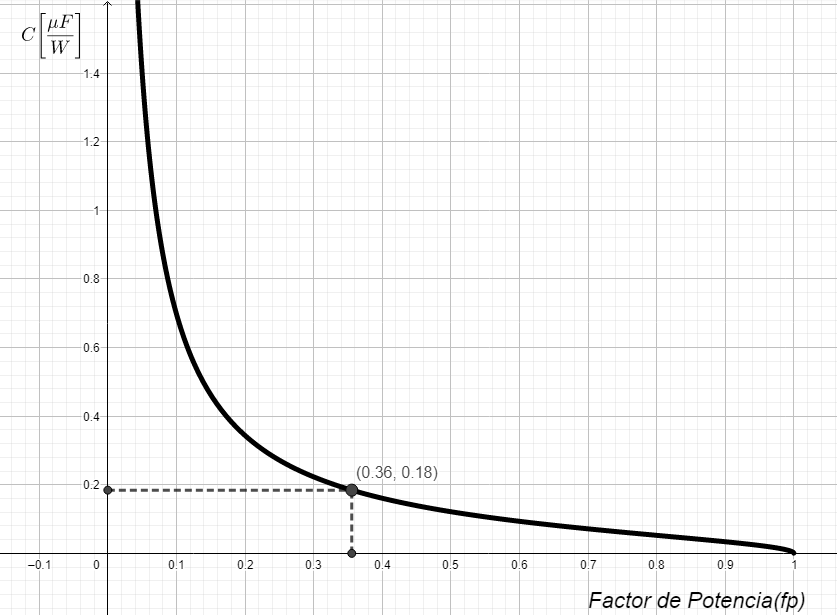
\includegraphics[width=0.7\textwidth]{Imagenes/ActividadPractica/CorreccionDeFdP/Curva Capa_FDP_Nueva.png}}
            \caption{Curva Capacitancia-Factor de Potencia.}
            \label{fig: Curva Cap_FDP}
        \end{figure}

        Para determinar el valor del capacitor de corrección mediante el gráfico, se debe 
        multiplicar el valor de la ordenada por la potencia activa medida.

    \subsubsection{Medición del factor de potencia corregido}\label{subsubsec:Medicion del factor de potencia corregido}

          Se dispone de un capacitor de valor $4,7~\mu F$, con lo cual se cumple el requisito presentado
          anteriormente, entonces se procede a la conexión del mismo, y a continuación se determina la nueva potencia aparente. 
          En la Figura \ref{fig: Señal_Correccion}, se visualiza el resultado de la modificación en el osciloscopio.
        
        \begin{figure}[H]
          \centering
          \frame{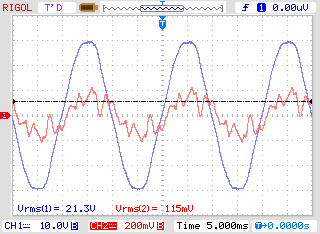
\includegraphics[width=0.45\textwidth]{Imagenes/ActividadPractica/CorreccionDeFdP/Exp2_11_Vin-Iin-ConCapacitor.png}}
          \caption{Señal resultante al agregar un capacitor.}
          \label{fig: Señal_Correccion}
        \end{figure}

        La señal resultante tiene una importante cantidad de armónicos sumados a la señal de corriente, ésto debido
        a la deformación provocada por la carga conectada a la red.

         Con los nuevos valores de tensión y corriente, se determina el valor de la nueva potencia 
         aparente

        \begin{align*}
          S = V\,I  = 213~V \cdot 0,115\ A \hspace{20pt} \Longrightarrow \hspace{20pt} \Aboxed{S = 24,50 ~[VA]}.
        \end{align*}

        Comparando éste último valor con el obtenido antes de corregir, 
        cuyo valor fué de $70.92~VA$, es notable la disminución de magnitud 
        de la potencia aparente al colocar en paralelo el capacitor.
        En éste caso, debido a la distorsión armónica, se complica bastante el 
        cálculo del factor de potencia, y en consecuencia de la potencia 
        activa y reactiva, por tal razón, éstas últimas no se calculan. No obstante, puede hacerse una mejor visualización 
        empleando los filtros del osciloscopio, lo cual no forma parte del 
        experimento, y se analizará más adelante.



        % Se tiene un semiperíodo de $10~ms$ (lo que se corresponde con la frecuencia de la red de $50~Hz$),
        % que equivalen a una pulsación de $180 ^{\circ}$, y usando la relación de tiempo/división del 
        % osciloscopio junto con la relación entre ángulo y tiempo, se determina de forma aproximada la correspondencia 
        % en grados del desfasaje de la señal

        % \begin{align*}
        %   \varphi = sen ^{-1} \left( \dfrac{t_{0} \cdot 180\ ^{\circ}}{0,5 \cdot T} \right) = sen ^{-1} \left( \dfrac{1,12~ms \cdot 180\ ^{\circ}}{10~ms} \right) \hspace{20pt} \Longrightarrow \hspace{20pt} \Aboxed{\varphi = 20,16\ ^{\circ}}\ .
        % \end{align*}    

   
